\chapter{CouchDB-Umfeld}
\label{Umfeld}

\section{Security}

\subsection{Absicherung des CouchDB-Servers}

Als moderne Management-Oberfläche für CouchDB steht die Web-Anwendung \emph{Fauxton} zur Verfügung. Diese bietet gleichzeitig den API-Zugang zur CouchDB für andere Anwendungen (in diesem Projekt die PouchDB-Anwendung). Diese kann einfach als npm-Paket installiert werden und ist danach über HTTP erreichbar \cite{fauxton:overview}. Welcher Webserver die Anwendung in diesem Fall ausliefert, ist nicht klar. Um nicht durch dessen eventuelle Sicherheitslücken gefährdet zu werden, muss zwischen diesen Webserver und das Internet ein sogenannter \emph{Reverse Proxy} geschaltet werden.

\begin{figure}[htb]
	\centering
	\caption{Netzwerkdiagramm für den Einsatz eines Reverse Proxy}
	\label{fig:reverseproxy}
	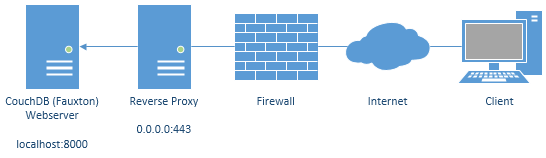
\includegraphics[width=\textwidth]{\figdir/Reverse_Proxy.png}
\end{figure}

Abbildung \ref{fig:reverseproxy} zeigt in einem Netzwerkdiagramm, wie der CouchDB-Server in diesem Projekt mit dem Internet verbunden ist. Eine Firewall lässt von außen nur Zugriffe über Port 443 (HTTPS) zu. Der Reverse Proxy lauscht an diesem Port und reicht alle Anfragen an den CouchDB/Fauxton-Webserver an Port 8000 weiter. Dabei wird gleichzeitig die TLS-Verbindung terminiert. Somit muss Fauxton keine TLS-Verbindungen aufbauen und braucht keine sicherheitskritischen Informationen über die verwendeten Zertifikate.

\subsection{Zugangskontrolle}

Der Zugang zu den Datenbanken auf dem CouchDB-Server muss durch Authentifizierung vor unbefugtem Zugriff geschützt werden. Zwar besitzt CouchDB ein Benutzer-Konzept, jedoch ist die Authentifizierung standardmäßig nicht aktiv:

\begin{citeenv}
	\begin{quotation}
		"`CouchDB has the idea of an admin user (e.g. an administrator, a super user, or root) that is allowed to do anything to a CouchDB installation. By default, everybody is an admin."' \cite{couch:security}.
	\end{quotation}
\end{citeenv}

Diese Standardeinstellung ist vor allem vor dem Hintergrund von 28.200 von Ransomware infizierten, ungesicherten MongoDB-Dokumentendatenbanken problematisch \cite{bleepingcomputer:mongodb:security}.

CouchDB kennt zwei unterschiedliche Benutzerrollen:

\begin{citeenv}
	\begin{quotation}
		\begin{itemize}
			\item \textit{members}, who are allowed to read all documents and create and modify any document except for design documents.
			\item \textit{admins}, who can read and write all types of documents, modify which users are members or admins, and set certain per-database configuration options.  \cite{couch:security}. (Hervorhebungen im Original)
		\end{itemize}
	\end{quotation}
\end{citeenv}

Damit lässt sich der unauthentifizierte Zugriff auf CouchDB-Datenbanken verhindern. Die Konfiguration erfolgt dabei mit JSON-Dokumenten in der \texttt{\_users}-Datenbank des Servers \cite{couch:security}. Benuterrollen für eine Datenbank können in einem jeweiligen Dokument namens \texttt{\_security} verwaltet werden.

% Todo: Quellen, Passwörter etc.